%%
%% Beginning of file 'sample.tex'
%%
%% Modified 2005 December 5
%%
%% This is a sample manuscript marked up using the
%% AASTeX v5.x LaTeX 2e macros.

%% The first piece of markup in an AASTeX v5.x document
%% is the \documentclass command. LaTeX will ignore
%% any data that comes before this command.

%% The command below calls the preprint style
%% which will produce a one-column, single-spaced document.
%% Examples of commands for other substyles follow. Use
%% whichever is most appropriate for your purposes.
%%
\documentclass[12pt,preprint]{aastex}

%% manuscript produces a one-column, double-spaced document:

%%\documentclass[manuscript]{aastex}

%% preprint2 produces a double-column, single-spaced document:

%% \documentclass[preprint2]{aastex}

%% Sometimes a paper's abstract is too long to fit on the
%% title page in preprint2 mode. When that is the case,
%% use the longabstract style option.

%% \documentclass[preprint2,longabstract]{aastex}

%% If you want to create your own macros, you can do so
%% using \newcommand. Your macros should appear before
%% the \begin{document} command.
%%
%% If you are submitting to a journal that translates manuscripts
%% into SGML, you need to follow certain guidelines when preparing
%% your macros. See the AASTeX v5.x Author Guide
%% for information.

\newcommand{\vdag}{(v)^\dagger}
\newcommand{\myemail}{skywalker@galaxy.far.far.away}

%% You can insert a short comment on the title page using the command below.

\slugcomment{Draft version}

%% If you wish, you may supply running head information, although
%% this information may be modified by the editorial offices.
%% The left head contains a list of authors,
%% usually a maximum of three (otherwise use et al.).  The right
%% head is a modified title of up to roughly 44 characters.
%% Running heads will not print in the manuscript style.

\shorttitle{A Study of the Point Spread Function at SDSS}
\shortauthors{Xin, Ivezi\'{c} and Friends}

%% This is the end of the preamble.  Indicate the beginning of the
%% paper itself with \begin{document}.

\begin{document}

%% LaTeX will automatically break titles if they run longer than
%% one line. However, you may use \\ to force a line break if
%% you desire.

\title{A Study of the Point Spread Function in SDSS Images}    %line break \\ is allowed in title


%% Use \author, \affil, and the \and command to format
%% author and affiliation information.
%% Note that \email has replaced the old \authoremail command
%% from AASTeX v4.0. You can use \email to mark an email address
%% anywhere in the paper, not just in the front matter.
%% As in the title, use \\ to force line breaks.

\author{B. Xin$^1$, \v{Z}. Ivezi\'{c}$^2$, R.H. Lupton$^3$, P. Yoachim$^2$, R.L. Jones$^2$, C. Claver$^1$, G. Angeli$^1$}
\and
\author{Other Contributors}

\affil{$^1$Large Synoptic Survey Telescope, Tucson, AZ 85719}
\affil{$^2$Department of Astronomy, University of Washington, Seattle, WA 98195}
\affil{$^3$Department of Astrophysical Sciences, Princeton University, Princeton, NJ 08544}



%\email{aastex-help@aas.org}


%% Mark off your abstract in the ``abstract'' environment. In the manuscript
%% style, abstract will output a Received/Accepted line after the
%% title and affiliation information. No date will appear since the author
%% does not have this information. The dates will be filled in by the
%% editorial office after submission.

\begin{abstract}
We use SDSS imaging data in $ugriz$ passbands to study the shape of
point spread function (PSF) profile and the variation of its width with 
wavelength and time. We find that the PSF profile is well described by 
theoretical predictions based on von Karman's turbulence theory and
can be parametrized by a single parameter, the profile's FWHM (full width
at half maximum). The profile shape is very similar to the ``double gaussian
plus power-law wing'' decomposition used by SDSS, but here it is modeled 
with a single free model parameter, rather than six as in SDSS pipeline. 
The FWHM variation with wavelength folows the
$\lambda^{-0.3}$ power law. We also measure the temporal and angular
structure functions for FWHM and find lots of interesting results \dots
\end{abstract}

%% Keywords should appear after the \end{abstract} command. The uncommented
%% example has been keyed in ApJ style. See the instructions to authors
%% for the journal to which you are submitting your paper to determine
%% what keyword punctuation is appropriate.

\keywords{imaging point spread function --- SDSS}

%% From the front matter, we move on to the body of the paper.
%% In the first two sections, notice the use of the natbib \citep
%% and \citet commands to identify citations.  The citations are
%% tied to the reference list via symbolic KEYs. The KEY corresponds
%% to the KEY in the \bibitem in the reference list below. We have
%% chosen the first three characters of the first author's name plus
%% the last two numeral of the year of publication as our KEY for
%% each reference.


%% Authors who wish to have the most important objects in their paper
%% linked in the electronic edition to a data center may do so by tagging
%% their objects with \objectname{} or \object{}.  Each macro takes the
%% object name as its required argument. The optional, square-bracket 
%% argument should be used in cases where the data center identification
%% differs from what is to be printed in the paper.  The text appearing 
%% in curly braces is what will appear in print in the published paper. 
%% If the object name is recognized by the data centers, it will be linked
%% in the electronic edition to the object data available at the data centers  
%%
%% Note that for sources with brackets in their names, e.g. [WEG2004] 14h-090,
%% the brackets must be escaped with backslashes when used in the first
%% square-bracket argument, for instance, \object[\[WEG2004\] 14h-090]{90}).
%%  Otherwise, LaTeX will issue an error. 

\section{Introduction}



ZI write a brief overview of SDSS and motivation for analysis (e.g. performance optimization
for LSST, \citealt{LSSToverview}): this shouldn't be hard and can be done in about a day. 

Hey Bo! Here is an example of using bibtex and cite call: SDSS PSF algorithm is described 
in \cite{Lupton2001}, \cite{Lupton2002}, and \citet[][see \S4.3]{SDSSEDR}.

Bo or ZI: add a brief summary with a few references (e.g. Young, Tyson, Roddier,
Tokovinin papers; can also recruit George for this part!) about what is known 
regarding:  PSF profile shape (e.g. Kolmogorov vs. von Karman), 
the dependence of FWHM on wavelength, and angular and temporal 
structure functions. 

Paper layout here.


\section{Data Overview} 

ZI's to do... 

\subsection{Stripe 82 dataset} 

ZI: why S82, what we used, data size...


\subsection{The treatment of seeing in SDSS}

ZI: steal the relevant text from the EDR paper (\citet{SDSSEDR}) and photo papers by \cite{Lupton2001} 
and \cite{Lupton2002}. 


\subsubsection{QA plots from SDSS Postage Stamp Pipeline (PSP)}

Testing (will probably be removed later): for each run, camera column and filter, PSP makes three QA plots, 
Figs.\ref{fig:PSPplot1}--\ref{fig:PSPplot3}. 


\begin{figure}
\centering
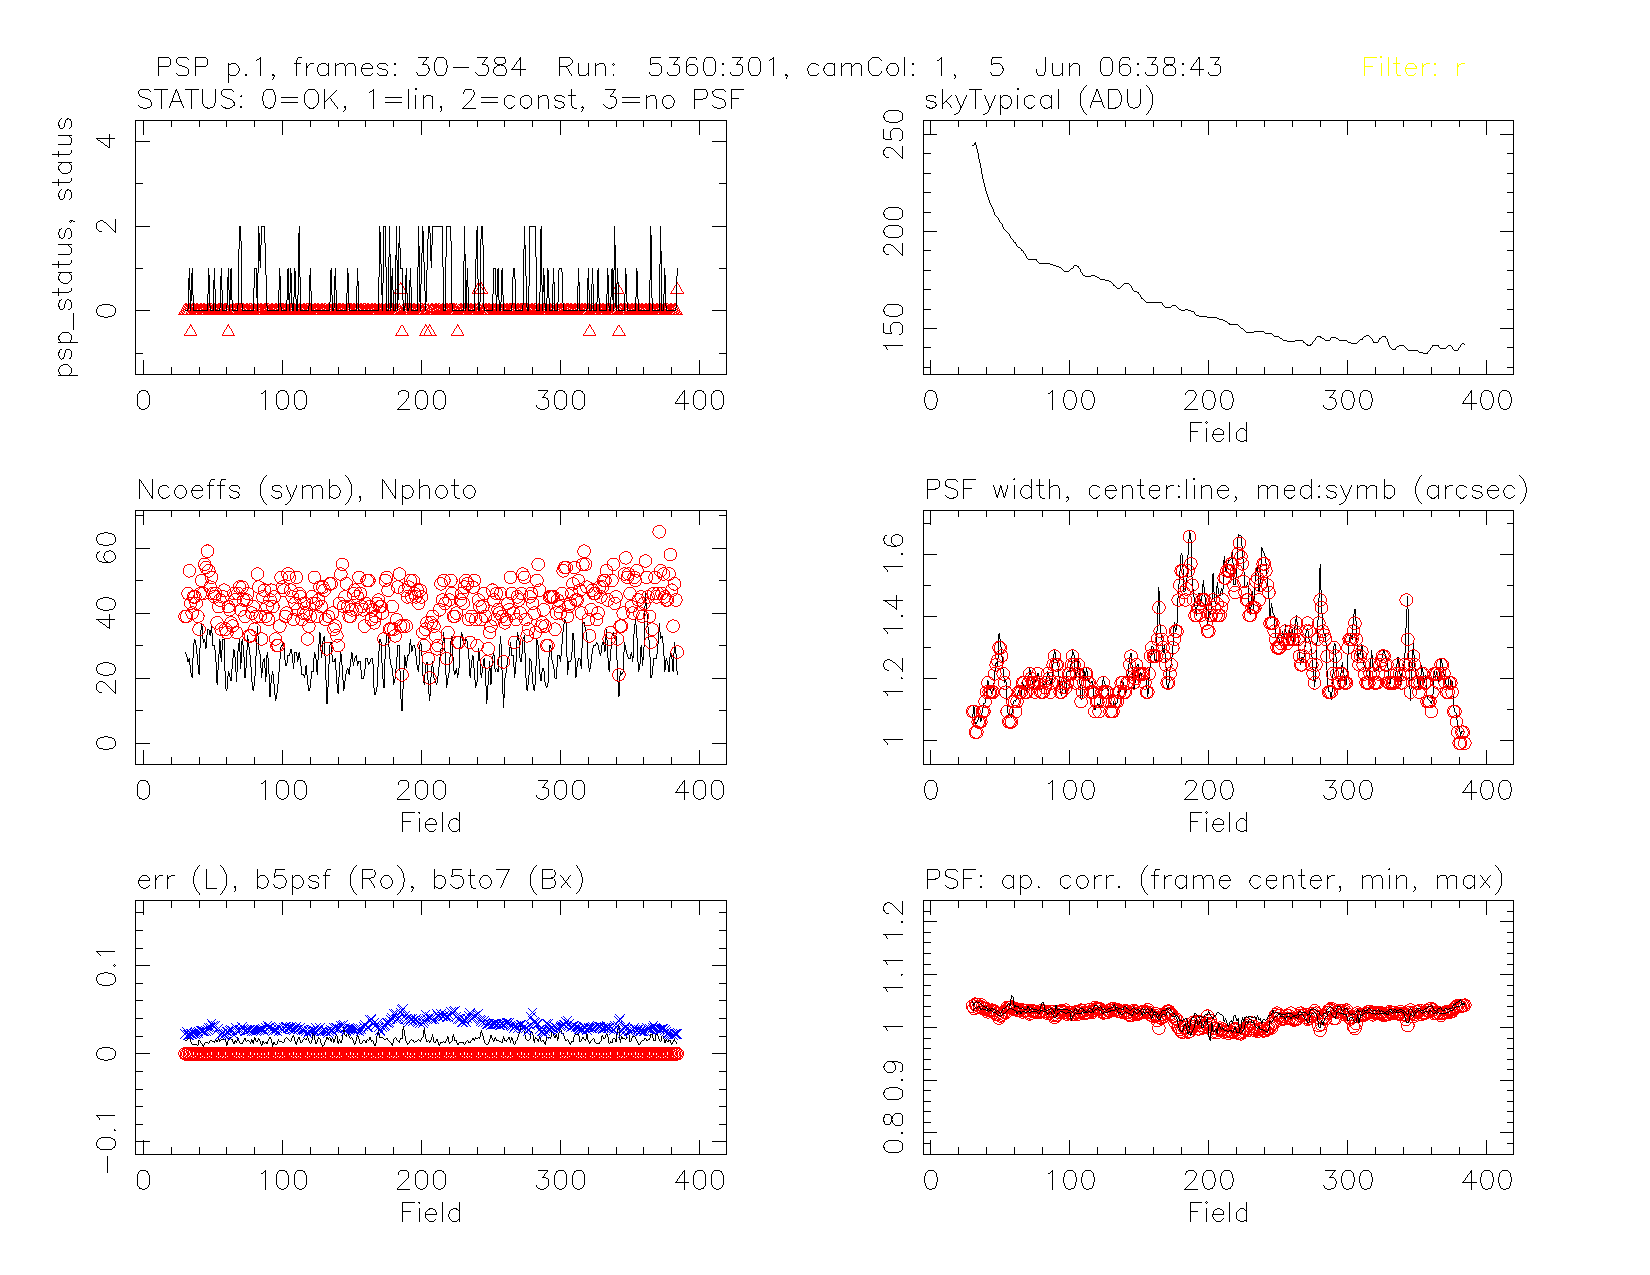
\includegraphics[width=0.9\textwidth]{FIGURES/psPlots1-005360-r1.pdf}
\caption{The plot 1 (psPlots1-005360-r1) produced by PSP for SDSS run 5306, 
camera column 1, in the $r$ band. The middle right panel shows the FWHM for
the measured seeing, as a function of field number (that is, as  function of time, 
with one field cooresponding to about 36 seconds). Note the large deterioration
of seeing between fields 130 and 300, lasting a bit under 2 hours. 
\label{fig:PSPplot1}}
\end{figure}


\begin{figure}
\centering
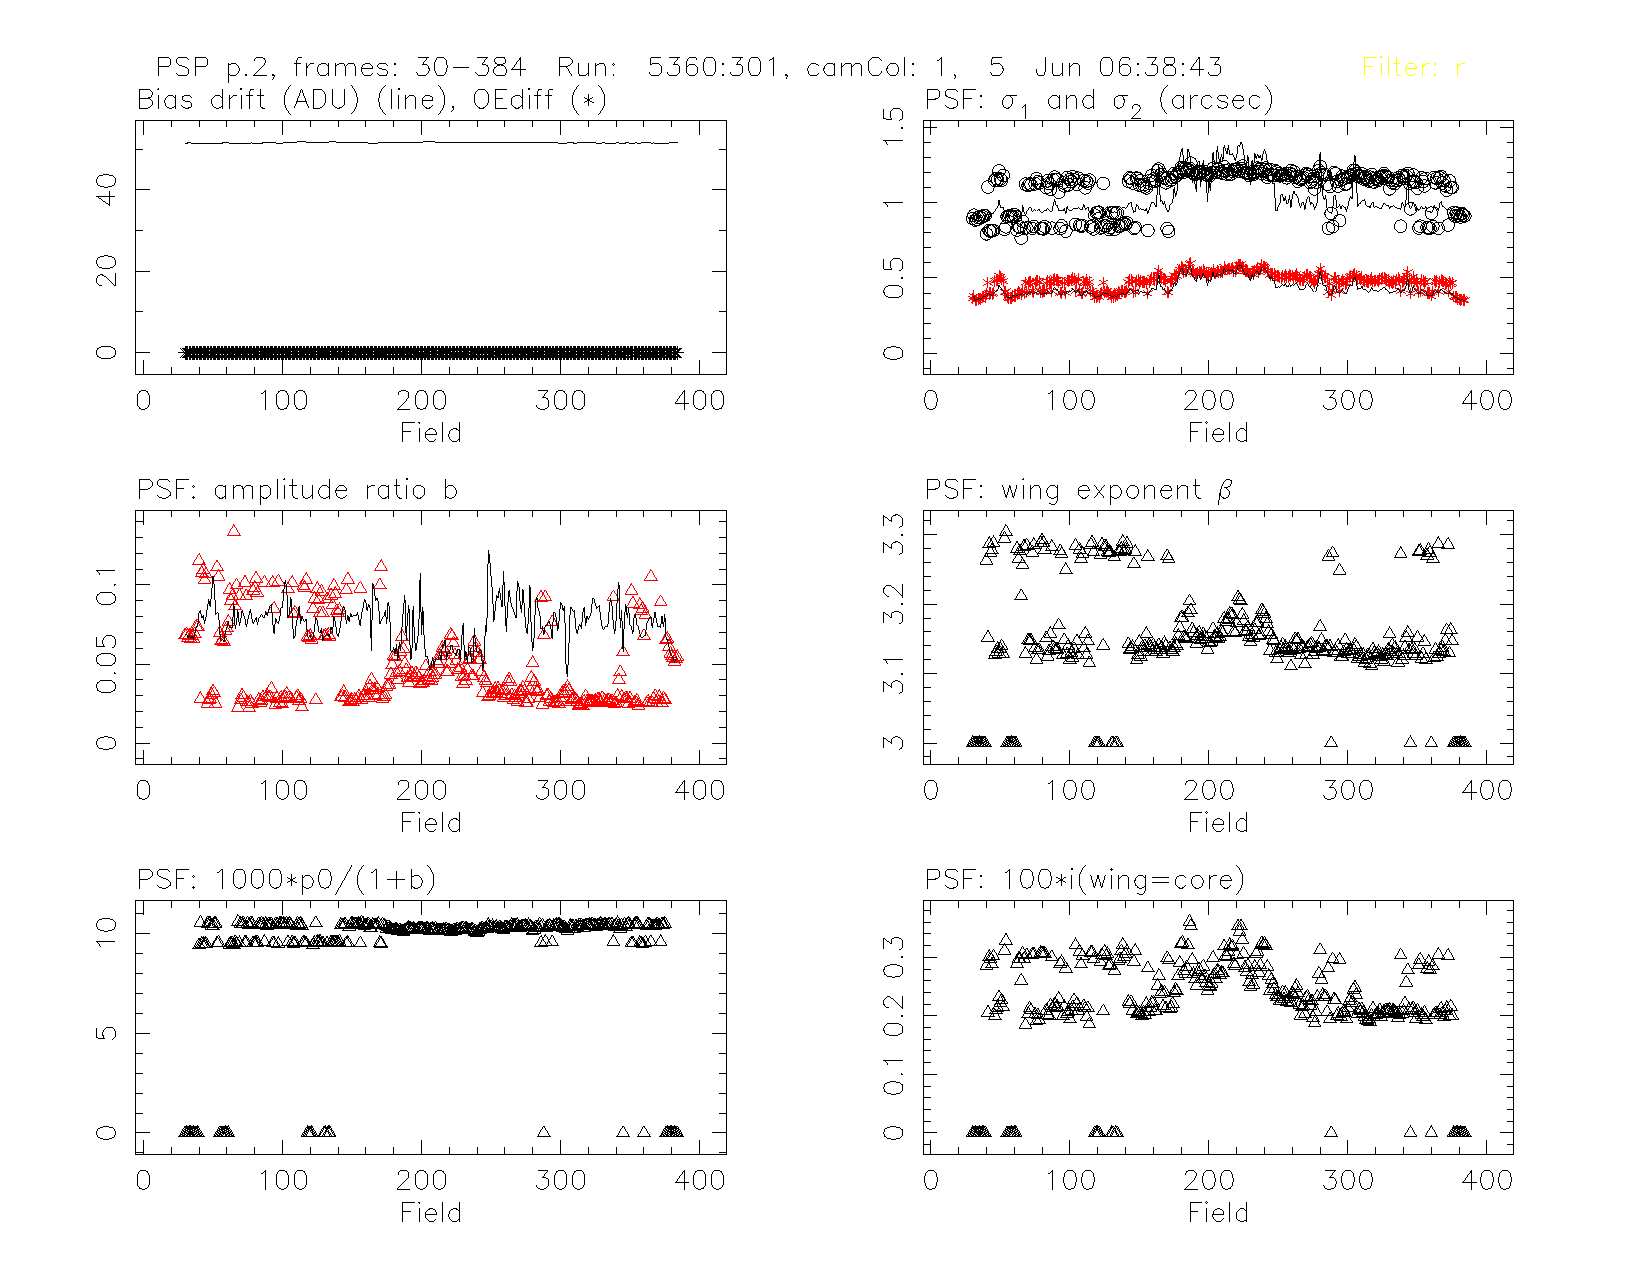
\includegraphics[width=0.9\textwidth]{FIGURES/psPlots2-005360-r1.pdf}
\caption{Similar to Fig~\ref{fig:PSPplot1}, except that here the plot 2 is shown.
Except for the top left panel, the best-fit PSF parameters (a double Gaussian
plus a power-law wing) are shown (see text for their description). 
\label{fig:PSPplot2}}
\end{figure}


\begin{figure}
\centering
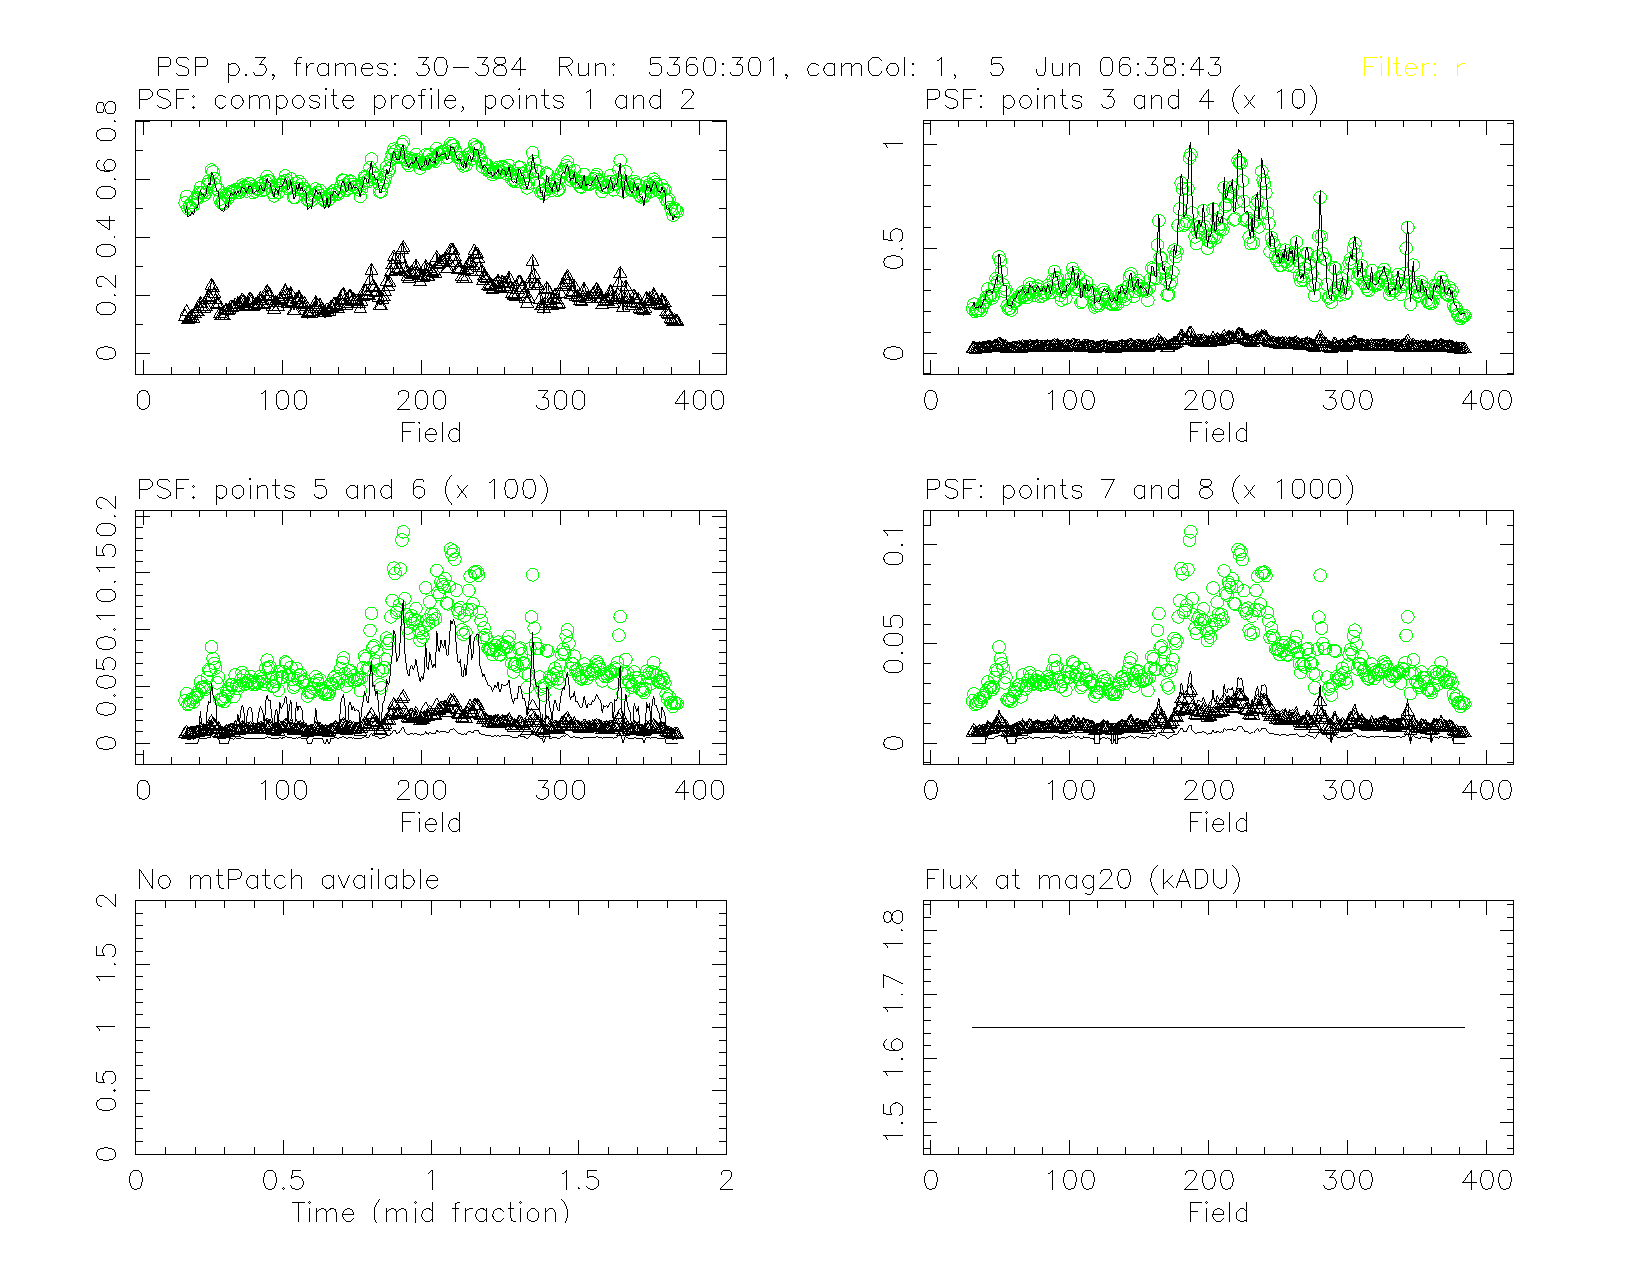
\includegraphics[width=0.9\textwidth]{FIGURES/psPlots3-005360-r1.pdf}
\caption{Similar to Fig~\ref{fig:PSPplot1}, except that here the plot 3 is shown.
The top four panels show the values of composite PSF profile (data).
\label{fig:PSPplot3}}
\end{figure}


\section{The PSF profile analysis}

Compare to SDSS, emphasize superiority of 1 parameter vs. 6 parameters fit

Discuss profile shape stability when the seeing is rapidly  changing 


\section{The analysis of FWHM behavior} 

Now that we understand (heopfully) that the seeing is by and large described by 
a single parameter, FWHM, we study three aspects of its variation, as follows.


\subsection{The FWHM dependence on wavelength} 

Asumming a power law, FWHM$\propto \lambda^{-\alpha}$, what can we say 
about $\alpha$ distribution? 


Why is SDSS PSF different for the $i$ band? The $i$ band psf has ``stronger tails''
becuse of scattering in the CCD.  The Si is transparent at long $i$-band wavelengths 
so light goes all the way through the chip and is reflected off the solder, and passes 
back up through the Si. This effect is not visible in the $z$ band because in this case
thick front-side chips are used (in all other bands, thin back-side chips are used). 


\subsection{Angular structure function} 

Cross-correlation of FWHM for 6 camera columns and the measurement of the angular
structure function (that is, the covariance vs. angular distance). 


\subsection{Temporal auto-correlation function}

Study the temporal power spectrum:
\begin{itemize}
\item Let's start with plain Fourier transform and look at power spectra (we can 
    play games with co-addition, 6 columns for a given run, or all runs)
\item Potentially, we could also look at  Kelly and Becker code  (2014, ApJ 788, 33) 
\item Here we can compare to Chuck's CP measurements (in opsim db) 
\end{itemize} 



\begin{table}[t!]
\caption{A little stolen table to test if it works here... It does! }
\vskip 0.05in
\begin{tabular}{|l|c|c|c|c|c|}
\hline  
    $r$   &  $\sigma^a_{xy} $  & $\sigma^b_\pi$  &   $\sigma^c_\mu$   &  $\sigma^d_1$  &  $\sigma^e_C$  \\
    mag &       mas            &      mas  & mas/yr &   mag   &    mag  \\
\hline  
       21 &  11  &  0.6  &  0.2   &   0.01  &   0.005 \\
       22 &  15  &  0.8  &  0.3   &   0.02  &   0.005 \\
       23 &  31  &  1.3  &  0.5   &   0.04  &   0.006 \\
       24 &  74  &  2.9  &  1.0   &   0.10  &   0.009 \\
\hline                         
\end{tabular}
\\ \vskip 0.05in
  $^a$ Typical astrometric accuracy (rms per coordinate per visit); \\
  $^b$ Parallax accuracy for 10-year long survey; \\
  $^c$ Proper motion accuracy for 10-year long survey; \\
  $^d$ Photometric error for a single visit (two 15-second exposures); \\
  $^e$ Photometric error for coadded observations (see Table 1). \\
\end{table}


\acknowledgments
We are grateful to George A. for buying us tamales and drinks. 


%% To help institutions obtain information on the effectiveness of their
%% telescopes, the AAS Journals has created a group of keywords for telescope
%% facilities. A common set of keywords will make these types of searches
%% significantly easier and more accurate. In addition, they will also be
%% useful in linking papers together which utilize the same telescopes
%% within the framework of the National Virtual Observatory.
%% See the AASTeX Web site at http://aastex.aas.org/
%% for information on obtaining the facility keywords.

%% After the acknowledgments section, use the following syntax and the
%% \facility{} macro to list the keywords of facilities used in the research
%% for the paper.  Each keyword will be checked against the master list during
%% copy editing.  Individual instruments or configurations can be provided 
%% in parentheses, after the keyword, but they will not be verified.

{\it Facilities:} \facility{SDSS}, \facility{LSST}.

%% Appendix material should be preceded with a single \appendix command.
%% There should be a \section command for each appendix. Mark appendix
%% subsections with the same markup you use in the main body of the paper.

%% Each Appendix (indicated with \section) will be lettered A, B, C, etc.
%% The equation counter will reset when it encounters the \appendix
%% command and will number appendix equations (A1), (A2), etc.

%\appendix
%
%\section{Appendix material}

%% The reference list follows the main body and any appendices.
%% Use LaTeX's thebibliography environment to mark up your reference list.
%% Note \begin{thebibliography} is followed by an empty set of
%% curly braces.  If you forget this, LaTeX will generate the error
%% "Perhaps a missing \item?".
%%
%% thebibliography produces citations in the text using \bibitem-\cite
%% cross-referencing. Each reference is preceded by a
%% \bibitem command that defines in curly braces the KEY that corresponds
%% to the KEY in the \cite commands (see the first section above).
%% Make sure that you provide a unique KEY for every \bibitem or else the
%% paper will not LaTeX. The square brackets should contain
%% the citation text that LaTeX will insert in
%% place of the \cite commands.

%% We have used macros to produce journal name abbreviations.
%% AASTeX provides a number of these for the more frequently-cited journals.
%% See the Author Guide for a list of them.

%% Note that the style of the \bibitem labels (in []) is slightly
%% different from previous examples.  The natbib system solves a host
%% of citation expression problems, but it is necessary to clearly
%% delimit the year from the author name used in the citation.
%% See the natbib documentation for more details and options.


\bibliographystyle{aj}
\bibliography{sdsspsf}


\end{document}



\begin{thebibliography}{}
\bibitem[Ivezi\'c et al. (2008)]{ivezic08} Ivezi\'c et al. 2008, arXiv:0805.2366v4
\end{thebibliography}


%% The following command ends your manuscript. LaTeX will ignore any text
%% that appears after it.

\end{document}

%%
%% End of file `sample.tex'.


1)  make files, one per run, as a function of field number, with
- field, camera column, bandpass, 
- one-parameter fit FWHM from fitting von Karman profile
- other SDSS params: psf_width, airmass, mjd, psf_nstar, neff_psf, sky_frames 


E.g. for some run
#  field  camCol  filter   FWHMvK    (other SDSS params)


2) plot FWHMvK vs. psf_width for 30 panels 

3) plot alpha (index for lambda dep.) histograms for all data and for 
    two realizations of ``longest stretch'' selection

4) plot profiles for a range of fields when the seeing is rapidly changing (is profile shape changing?) 


Also: 
ZI:  find exact definition of neff_psf (is it based on fit or input data?) 
Bo: add analysis directory and py code 


Analysis structure:

1) profile discussion
- compare to SDSS, emphasize 1 parameter vs. 6 parameters
- discuss profile shape stability when seeing is changing rapidly

2) dependence on wavelength

- what is alpha distribution? 

3) cross-correlation of camera columns and measurement of structure function
    (that is, the covariance vs. angular distance) 

4) auto-correlation function (and power spectrum) for temporal variation

- let's start with plain Fourier transform and look at power spectra (we can 
    play games with co-addition, 6 columns for a given run, or all runs)
- potentially, we could also look at  Kelly and Becker code  (2014, ApJ 788, 33) 
- here we can compare to Chuck's CP measurements (in opsim db) 
